\documentclass[border=5pt]{standalone}
\usepackage{pgfplots}
\pgfplotsset{compat=1.18}
\usepackage{amsmath}
\begin{document}
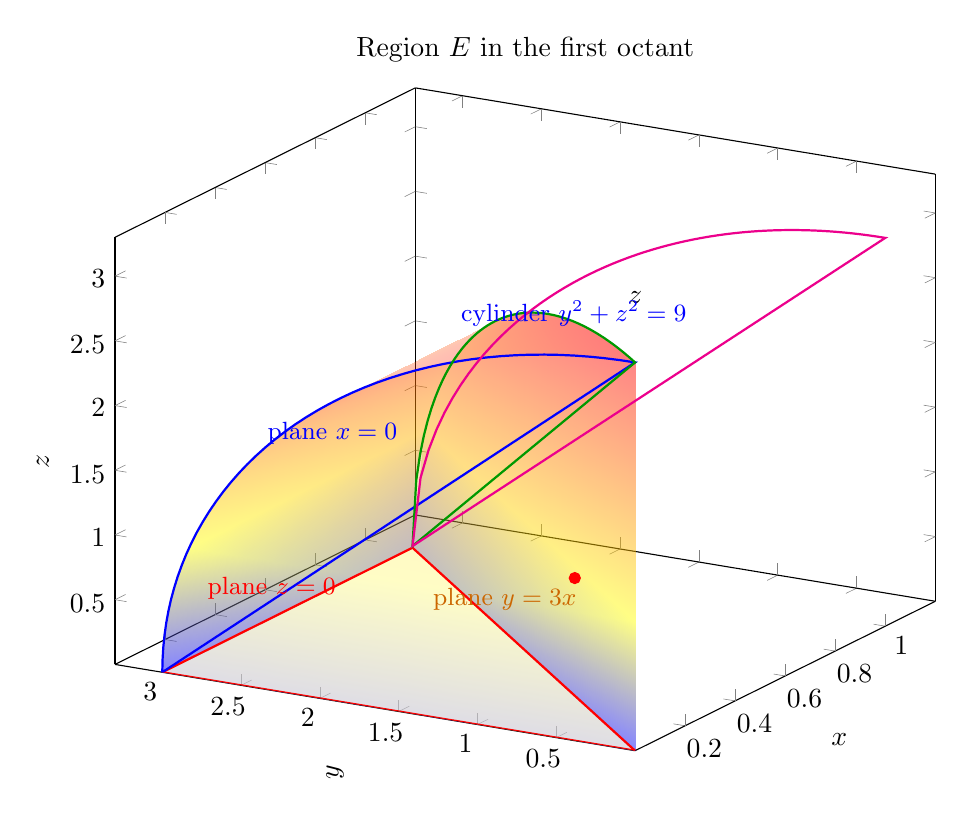
\begin{tikzpicture}
\begin{axis}[
    view={-60}{22},
    xlabel={$x$}, ylabel={$y$}, zlabel={$z$},
    xmin=0, xmax=1.2,
    ymin=0, ymax=3.3,
    zmin=0, zmax=3.3,
    xtick={0.2,0.4,0.6,0.8,1.0},
    ytick={0.5,1.0,1.5,2.0,2.5,3.0},
    ztick={0.5,1.0,1.5,2.0,2.5,3.0},
    axis lines=box,
    width=12cm, height=10cm,
    title={Region $E$ in the first octant},
    legend style={font=\footnotesize}
]

% Cylinder surface y^2+z^2=9 within first octant
% Parametrize: x in [0,1], theta in [0,pi/2]
\addplot3[
    surf, shader=interp,
    mesh/ordering=y varies,
    domain=0:1, y domain=0:1.5708,
    samples=25, samples y=30,
    z buffer=sort,
    opacity=0.30, fill=blue!30
] (
    {min(x, cos(deg(y)))},
    {3*cos(deg(y))},
    {3*sin(deg(y))}
);

% Slanted plane y = 3x within cylinder
\addplot3[
    surf, shader=interp,
    mesh/ordering=y varies,
    domain=0:1, y domain=0:3,
    samples=20, samples y=20,
    opacity=0.30, fill=orange!40
] ({x}, {3*x}, {min(y, sqrt(9 - 9*x^2))});

% Back wall (x = 0) quarter disk
\addplot3[
    surf, shader=interp,
    domain=0:1.5708, y domain=0:1,
    samples=25, samples y=5,
    opacity=0.25, fill=gray!30
] (0, {3*cos(deg(x))}, {3*sin(deg(x))*y});

% Bottom triangle (z=0): vertices (0,0,0), (0,3,0), (1,3,0)
\addplot3[
    fill=yellow!20, opacity=0.5
] coordinates {(0,0,0) (0,3,0) (1,3,0)} -- cycle;

% Sharp edges
% Edge along y=3x in z=0 plane (red)
\addplot3[red, thick] coordinates {(0,0,0) (1,3,0)};
% Edge along x=0, z=0 (red)
\addplot3[red, thick] coordinates {(0,0,0) (0,3,0)};
% Edge along y=3, z=0 (red)
\addplot3[red, thick] coordinates {(0,3,0) (1,3,0)};
% Back quarter circle x=0 (blue)
\addplot3[blue, thick, samples=50, domain=0:1.5708, variable=t]
    (0, {3*cos(deg(t))}, {3*sin(deg(t))});
% Top curve where cylinder meets slanted plane (green)
\addplot3[green!60!black, thick, samples=60, domain=0:3, variable=y]
    ({y/3}, {y}, {sqrt(9 - y^2)});
% Curve at x = 1 (magenta)
\addplot3[magenta, thick, samples=60, domain=0:3, variable=y]
    (1, {y}, {sqrt(9 - y^2)});

% Sample point
\addplot3[only marks, mark=*, mark size=2pt, red] coordinates {(0.2, 0.7, 1.0)};

% Axis labels
\node at (axis cs:1.4,0,0) {$x$};
\node at (axis cs:0,3.5,0) {$y$};
\node at (axis cs:0,0,3.5) {$z$};

% Annotations
\node[blue] at (axis cs:0.7, 1.5, 2.4) {\small cylinder $y^2+z^2=9$};
\node[orange!80!black] at (axis cs:0.55, 1.7, 0.3) {\small plane $y=3x$};
\node[red] at (axis cs:0.5, 3.1, 0.15) {\small plane $z=0$};
\node[blue] at (axis cs:0.05, 2.0, 2.0) {\small plane $x=0$};

\end{axis}
\end{tikzpicture}
\end{document}